% vim: set spell spelllang=es syntax=tex :

\section{Fútbol de robots}

La \emph{RoboCup} \cite{robocupHist} (del inglés \emph{Robot World Cup}) es una
competencia internacional celebrada desde 1997, donde equipos de robots juegan
una versión simplificada del fútbol. Su finalidad es la de ofrecer un ambiente
controlado donde poner a prueba los avances en distintas áreas de conocimiento
como la inteligencia artificial, visión por computadora y robótica. Existen
cinco ligas distintas cuyas características varían desde la simulación del
ambiente y robots, hasta robots humanoides con visión local. De éstas, la más
antigua es la liga de tamaño pequeño (\emph{SSL}, del inglés \emph{Small Size
League}).

Nota de OSO: Se puede agregar info detallada de cada una de las ligas

Un partido de la \emph{SSL} enfrenta a dos equipos de seis robots, que deben
tener un tamaño menor que un cilindro de 9$cm$ de radio y 15$cm$ de
alto \cite{sslrules2015}, se movilizan sobre ruedas y tienen un ``pie'' con el
que patear la pelota. Los detalles de su construcción no están reglamentados,
aunque los equipos suelen coincidir en algunos puntos, como por ejemplo el uso
de ruedas omnidireccionales.

Cada equipo cuenta con una computadora fuera del campo de juego, a la cual se
delega la toma de decisiones y planeamiento del movimiento de los robots. Por
su parte la capacidad de procesamiento de los robots se limita a aquella
necesaria para ejecutar las ordenes de movimiento de la computadora de su
equipo. Estas computadoras perciben el ambiente a través de un sistema de
visión global centralizado compartido. Se utiliza un conjunto de cámaras,
montadas sobre distintas áreas del campo de juego y conectadas a una
computadora donde se ejecuta el sistema de visión. El sistema detecta la
posición y orientación de cada uno de los robots y la posición de la pelota, y
reporta esta información a las computadoras que controlan los equipos.

Para que el sistema de visión pueda identificar a cada robot, cada uno tiene
sobre su parte superior cinco parches de colores. El parche que se encuentra
en el centro indica el color del equipo del robot, y los cuatro restantes
sirven para identificar al robot dentro del equipo y para conocer la
orientación que lleva en cada momento. La pelota es de un color uniforme y
distinto al de los parches de los robots; normalmente, naranja, ya que este
color contrasta fácilmente con el verde de la cancha. En la figura
\ref{sistemaVG} se muestra la arquitectura del sistema con tres robots, dos
del equipo azul y uno del equipo rojo.

\begin{figure}[!h]

	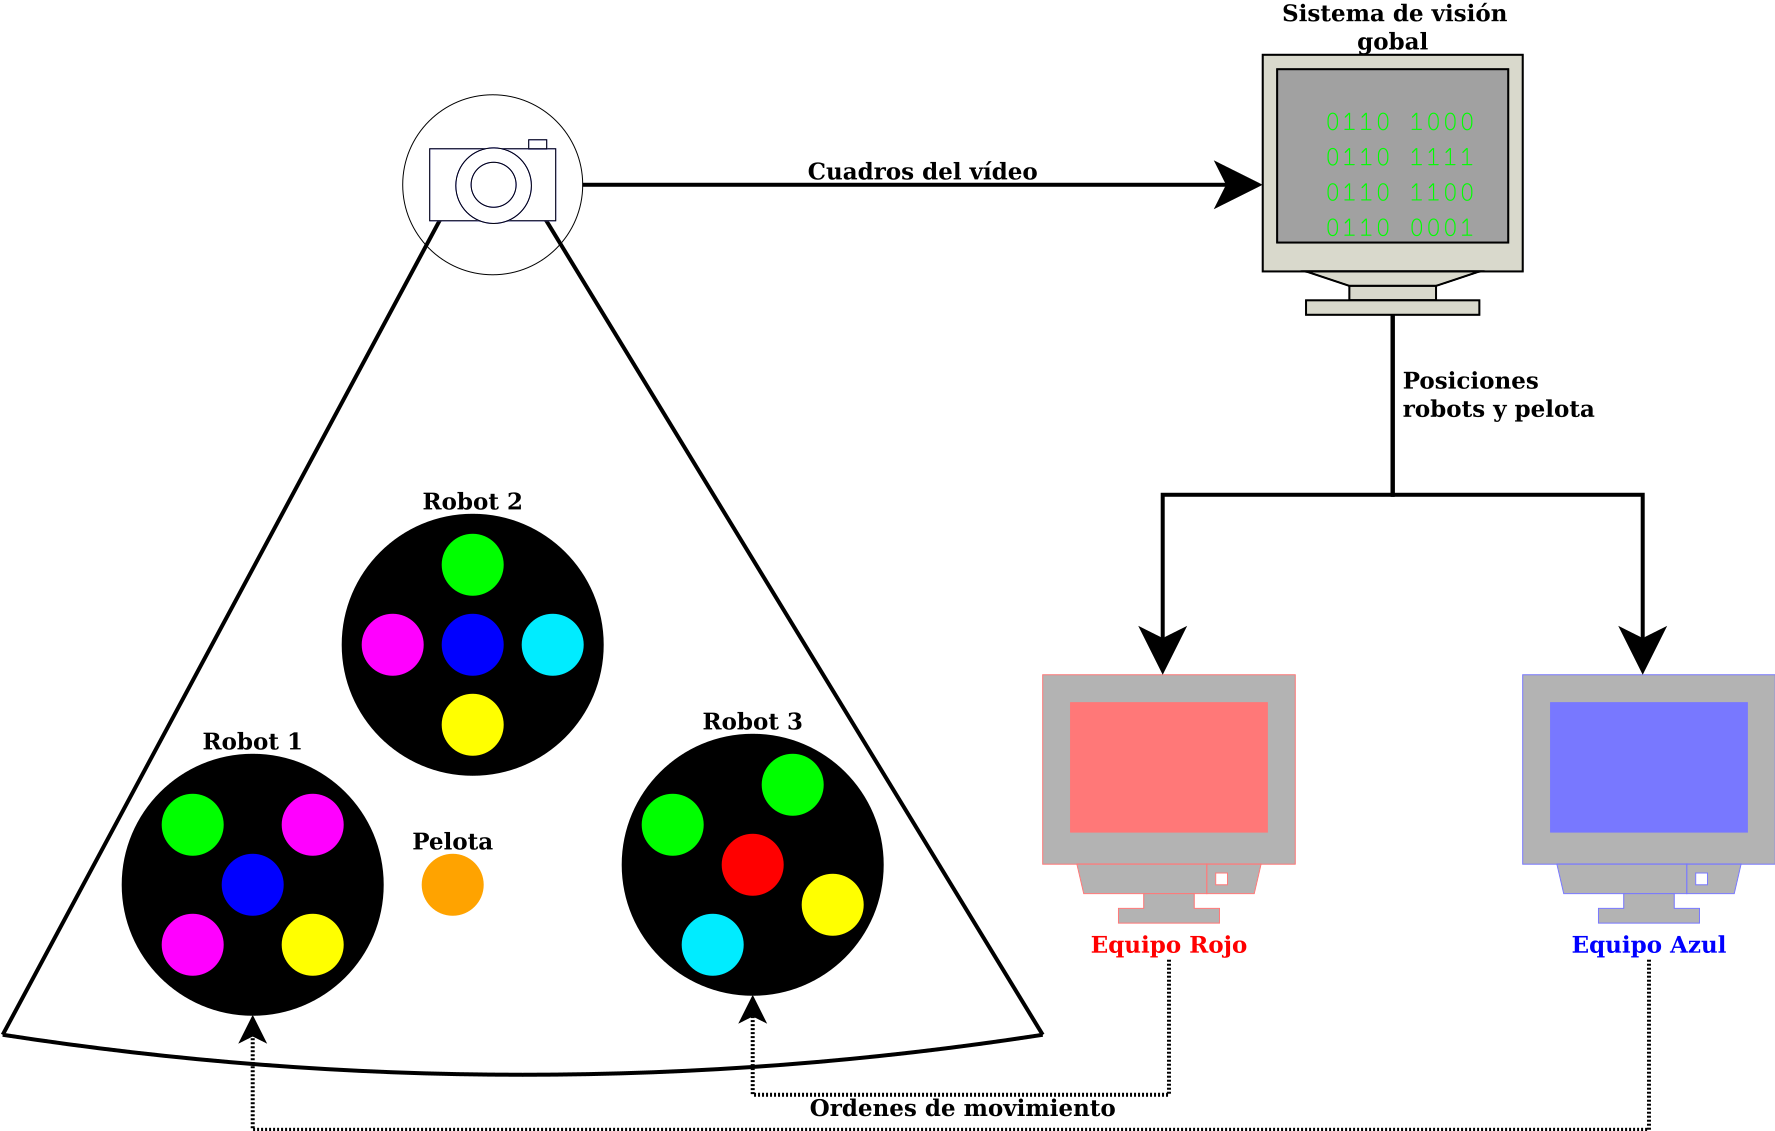
\includegraphics[width=\textwidth]{img/sistemaVG.pdf}

	\caption{Estructura de comunicación del sistema de visión global en
	fútbol de robots de la \emph{SSL}.}

	\label{sistemaVG}

\end{figure}

El uso de este sistema centralizado permite a los participantes abstraerse de
los problemas de la visión por computadora y enfocarse en la estrategia del
juego. Además, permite que las tareas de calibración y montaje de las cámaras se
realicen una sola vez para cada campo de juego, en vez de para cada partido.

Las computadoras utilizadas para la ejecución del sistema de visión global son
equipos de escritorio de gama media o alta. Esto permite que el sistema pueda
ser ejecutado en el sitio donde se lleva a cabo el partido de la \emph{SSL} y
aumenta la cantidad de equipos de hardware disponibles.

El fútbol de robots se desarrolla en un contexto de tiempo real, ya que el
ciclo completo de procesamiento de información debe cumplirse en un plazo
máximo para poder alcanzar los objetivos.  El servidor debe procesar cada
cuadro para entregar la información de posición y velocidad de cada elemento
en el campo de juego a las computadoras coordinadoras de los equipos; y éstas
deben tomar una decisión y comunicarla a los robots, todo dentro de un tiempo
de respuesta razonable para el progreso de la aplicación.

Los parámetros de calidad de este tipo de sistema son, normalmente:

\begin{itemize}

	\item 	tasa de aciertos en la detección de objetos;

	\item 	precisión en la posición y orientación de los aciertos en la
		detección de objetos;

	\item 	precisión en la posición y orientación de los robots y pelota;

	\item 	cuadros por segundo (\emph{FPS}, del inglés \emph{Frames Per
		Second}) procesados;

	\item 	y máximo tiempo de espera del cuadro (tiempo desde la creación
		del cuadro hasta la entrega de la información extraída).

\end{itemize}

Originalmente el tamaño de la cancha era de 4,9$m\times$3,4$m$, lo que
permitía que todo el campo de juego fuera observado con una sola cámara. Luego
se optó por dos tipos de canchas en los partidos de la \emph{SSL}: las canchas
de tamaño simple, con un tamaño de 6,05$m\times$4,05$m$ para las cuales se
utilizan dos cámaras, una sobre cada media cancha, y las de tamaño doble, con
un tamaño de 8,09$m\times$6,05$m$, que utilizan cuatro cámaras, una por cada
mitad de cada media cancha. Desde el año 2015, las canchas de tamaño doble son
las utilizadas de forma predeterminada \cite{sslrules2015}. Con este cambio se
espera permitir la exploración de nuevas tácticas por parte de los equipos, ya
que una mayor área de juego permite a los robots movimientos de mayor amplitud
y variedad. En la figura \ref{cancha} se muestran los tamaños de las canchas y
la distribución de las cámaras.

\begin{figure}[!h]

	\centering

	\begin{subfigure}[c]{0.45\textwidth}
		\centering
		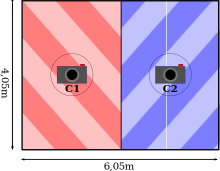
\includegraphics[scale=0.8]{img/cancha605cm.pdf}
		\caption{}
	\end{subfigure}
	~
	\begin{subfigure}[c]{0.45\textwidth}
		\centering
		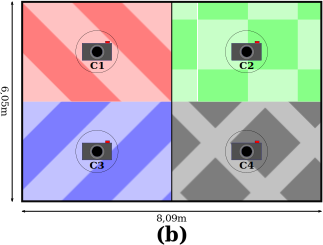
\includegraphics[scale=0.8]{img/cancha809cm.pdf}
		\caption{}
	\end{subfigure}

	\caption{Dimensiones y área de cobertura de las cámaras en la liga
	\emph{SSL}, en competencias a) anteriores a 2015; b) año 2015 y
	posteriores.}

	\label{cancha}

\end{figure}

Sin embargo, como consecuencia, en las canchas de tamaño doble, el sistema de
visión debe procesar cuatro veces más información que en las canchas
originales y el doble que las canchas de tamaño doble, lo que da lugar a un
problema para un sistema de tiempo real como este. El aumento en la cantidad
de información impacta negativamente en el rendimiento debido a que se reducen
los cuadros por segundo procesados y se incrementa el tiempo de espera del
cuadro.

Como se utilizan computadoras de escritorio convencionales para la ejecución
del sistema de visión global es sensato asumir que se trata de un sistema de
memoria compartida de múltiples núcleos\footnote{Según la encuesta de hardware
de la plataforma de distribución digital \emph{Steam} de marzo del 2017
\cite{steamSurvey}, solo el $1.93$\% de los equipos donde esta instalado posee
un solo núcleo.}, pero el sistema actual utilizado por la \emph{SSL} ejecuta
en un solo hilo, aprovechando solo uno de los núcleos disponibles. Por esto se
plantea como posibilidad crear un nuevo sistema de visión global paralelo con
el fin de aumentar el rendimiento del sistema al hacer un mayor uso de los
recursos disponibles.
